\documentclass{beamer}
\usepackage{ctex}
\usepackage{minted}
\usetheme{metropolis}           % Use metropolis theme
\title{Flink流处理简介}
\date{\today}
\author{左元}
\institute{尚硅谷 大数据组}
\begin{document}
  \maketitle
  \begin{frame}{主要内容}
    \begin{itemize}
      \item Flink是什么
      \item 为什么要用Flink
      \item 流处理的发展和演变
      \item Flink的主要特点
      \item Flink vs Spark Streaming
    \end{itemize}
  \end{frame}

  \begin{frame}{Flink是什么}
    \begin{figure}
        \centering
        \begin{minipage}{0.45\textwidth}
            \centering
            
\includegraphics[width=0.9\textwidth, height=0.4\textheight]{image1.png} % first figure itself
            \caption{Apache Logo}
        \end{minipage}\hfill
        \begin{minipage}{0.45\textwidth}
            \centering
            
\includegraphics[width=0.9\textwidth, height=0.4\textheight]{image2.png} % second figure itself
            \caption{Flink Logo}
        \end{minipage}
    \end{figure}
    \begin{itemize}
      \item Apache Flink is a framework and distributed processing engine for stateful computations over unbounded and bounded data streams.
      \item Apache Flink 是一个\textcolor{red}{框架}和\textcolor{red}{分布式}处理引擎,用于对\textcolor{red}{无界和有界数据流}进行\textcolor{red}{状态}计算。
    \end{itemize}
  \end{frame}

  \begin{frame}
    \frametitle{Flink目前在国内企业的应用}
  
    \begin{figure}
      \centering
      
\includegraphics[width=0.9\textwidth]{image3.png}
      \caption{Flink目前在国内企业的应用}
    \end{figure}
  
  \end{frame}

  \begin{frame}{为什么选择Flink}
    \begin{itemize}
      \item 流数据更真实地反映了我们的生活方式
      \item 传统的数据架构是基于有限数据集的
      \item 我们的目标
        \begin{itemize}
          \item 低延迟(Spark Streaming的延迟是秒级,Flink延迟是毫秒级)
          \item 高吞吐(阿里每秒钟使用Flink处理4.6PB,双十一大屏)
          \item 结果的准确性和良好的容错性(exactly-once)
        \end{itemize}
    \end{itemize}
  \end{frame}

  \begin{frame}
    \frametitle{哪些行业需要处理流数据}
  
    \begin{itemize}
      \item 电商和市场营销
        \begin{itemize}
          \item 数据报表、广告投放、业务流程需要
        \end{itemize}
      \item 物联网(IOT)
        \begin{itemize}
          \item 传感器实时数据采集和显示、实时报警,交通运输业(自动驾驶)
        \end{itemize}
      \item 电信业
        \begin{itemize}
          \item 基站流量调配
        \end{itemize}
      \item 银行和金融业
        \begin{itemize}
          \item 实时结算和通知推送,实时检测异常行为(信用卡盗卡)
        \end{itemize}
    \end{itemize}
  \end{frame}

  \begin{frame}
    \frametitle{传统数据处理架构}
  
    \begin{itemize}
      \item 事务处理(OLTP)
    \end{itemize}

    \begin{figure}
      \centering
      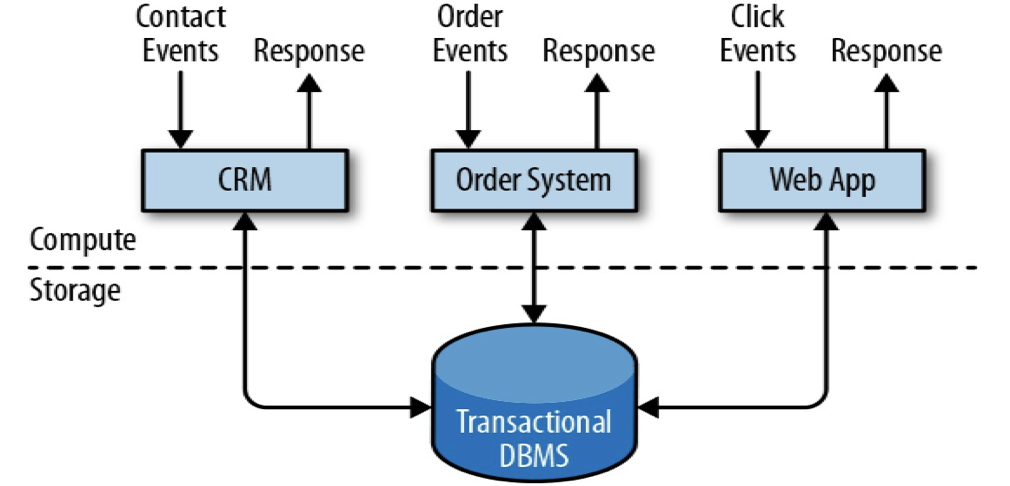
\includegraphics[width=0.9\textwidth]{image4.png}
      \caption{OLTP架构}
    \end{figure}
  
  \end{frame}

  \begin{frame}
    \frametitle{传统数据处理架构}
  
    \begin{itemize}
      \item 分析处理
        \begin{itemize}
          \item 将数据从业务数据库复制到数仓,再进行分析和查询
        \end{itemize}
    \end{itemize}

    \begin{figure}
      \centering
      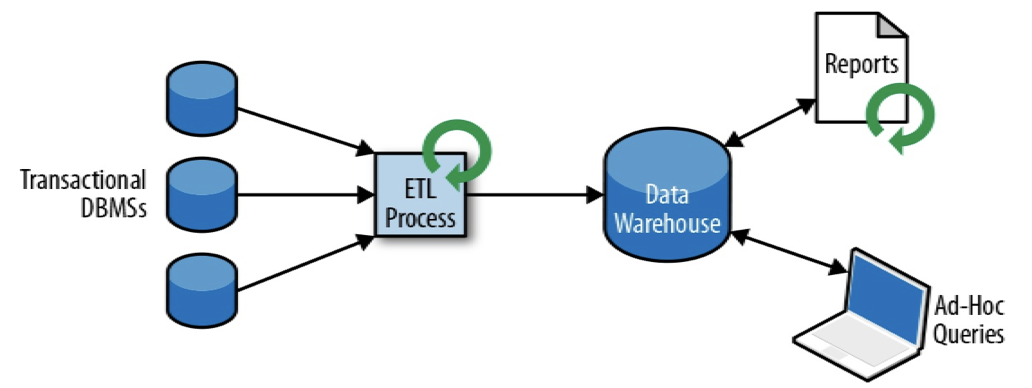
\includegraphics[width=0.9\textwidth]{image5.png}
      \caption{OLAP架构}
    \end{figure}
  
  \end{frame}

  \begin{frame}
    \frametitle{有状态的流式处理}

    \begin{figure}
      \centering
      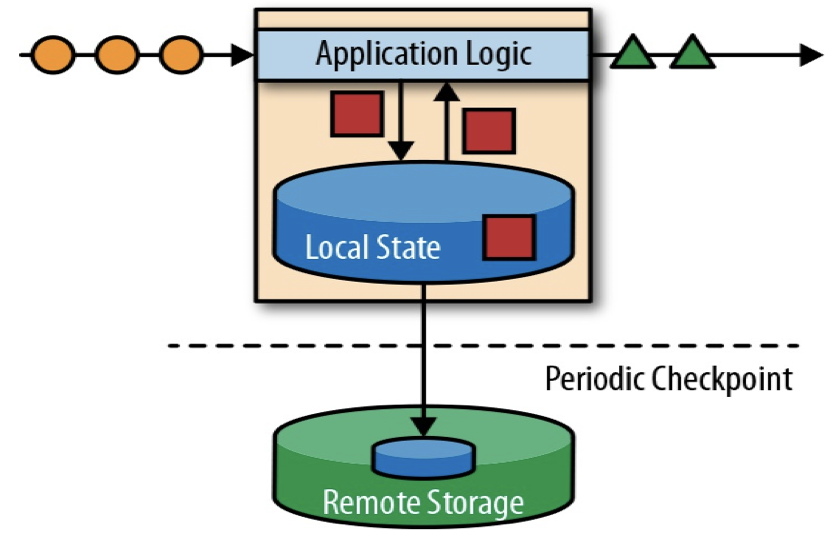
\includegraphics[width=0.9\textwidth]{image6.png}
      \caption{有状态的流式处理}
    \end{figure}
  
  \end{frame}

  \begin{frame}
    \frametitle{流处理的演变}
  
    \begin{itemize}
      \item lambda 架构
        \begin{itemize}
          \item 用两套系统,同时保证低延迟和结果准确
        \end{itemize}
    \end{itemize}

    \begin{figure}
      \centering
      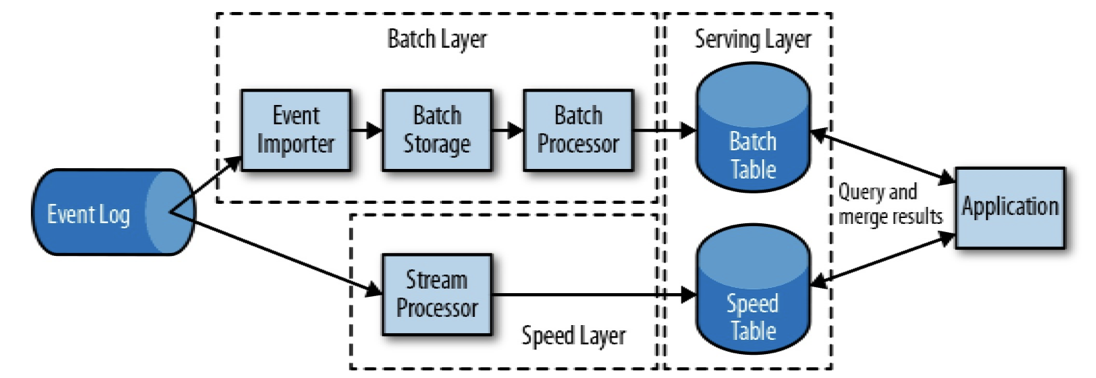
\includegraphics[width=0.9\textwidth]{image7.png}
      \caption{lambda架构}
    \end{figure}
  
  \end{frame}

  \begin{frame}
    \frametitle{流处理的演变}
  
    \begin{figure}
      \centering
      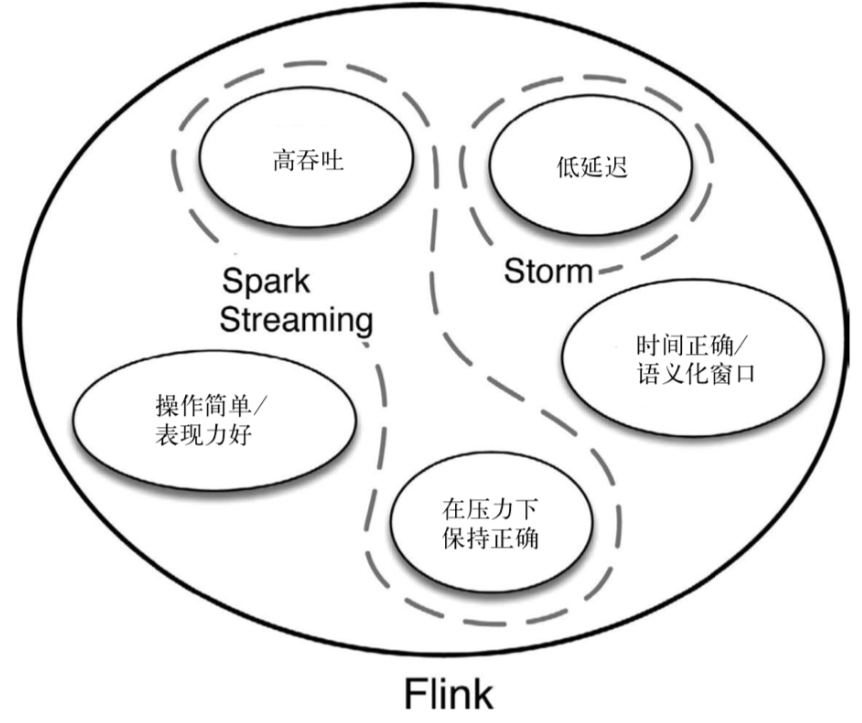
\includegraphics[width=0.9\textwidth]{image8.png}
      \caption{流处理的演变}
    \end{figure}
  
  \end{frame}

  \begin{frame}
    \frametitle{Flink的主要特点}
  
    \begin{itemize}
      \item 事件驱动(Event-driven)
    \end{itemize}

    \begin{figure}
      \centering
      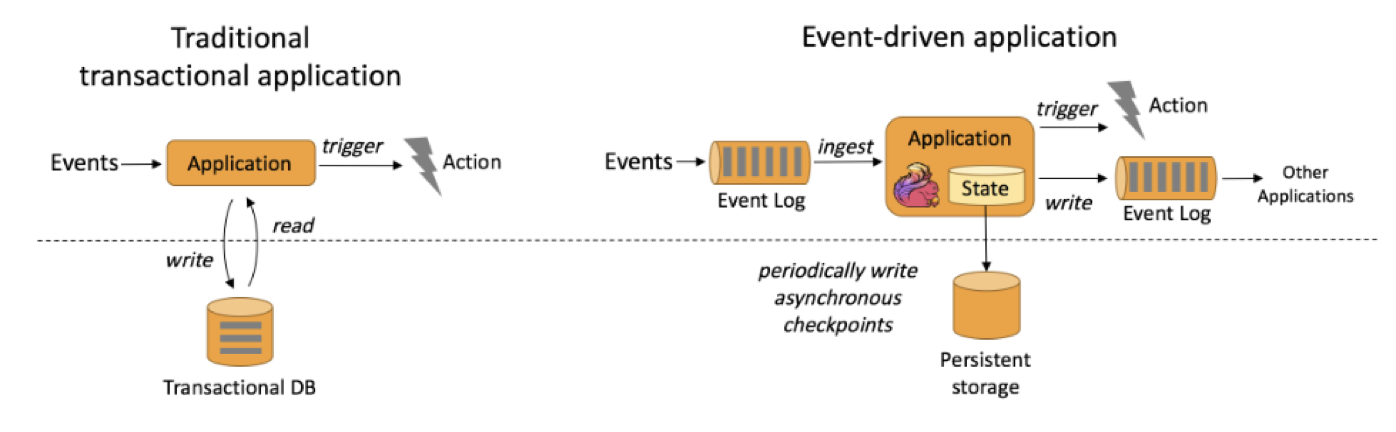
\includegraphics[width=0.9\textwidth]{image9.png}
      \caption{事件驱动}
    \end{figure}
  
  \end{frame}

  \begin{frame}
    \frametitle{Flink的主要特点}
  
    \begin{itemize}
      \item 基于流的世界观
        \begin{itemize}
          \item 在 Flink 的世界观中,一切都是由流组成的,离线数据是有界的流;实时数据是一个没有界限的流:这就是所谓的有界流和无界流
        \end{itemize}
    \end{itemize}

    \begin{figure}
      \centering
      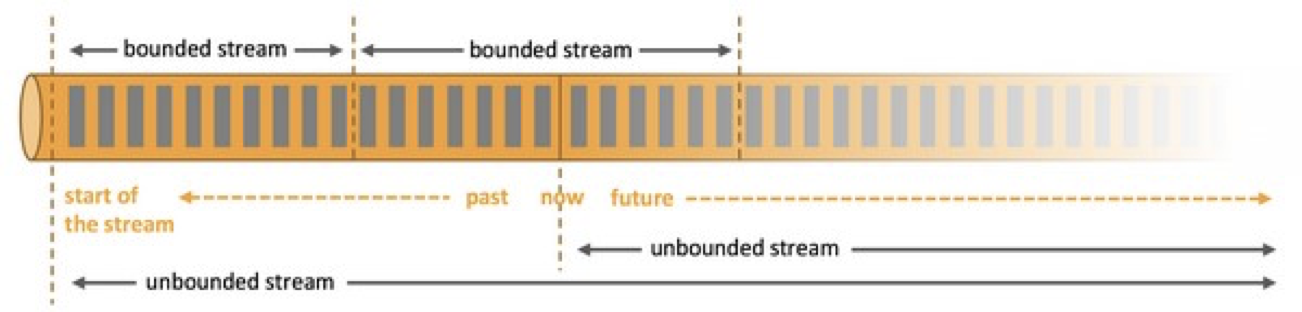
\includegraphics[width=0.9\textwidth]{image10.png}
      \caption{流批统一}
    \end{figure}
  
  \end{frame}

  \begin{frame}
    \frametitle{Flink的主要特点}
  
    \begin{itemize}
      \item Flink的分层API
        \begin{itemize}
          \item 越顶层越抽象,表达含义越简明,使用越方便
          \item 越底层越具体,表达能力越丰富,使用越灵活
        \end{itemize}
    \end{itemize}

    \begin{figure}
      \centering
      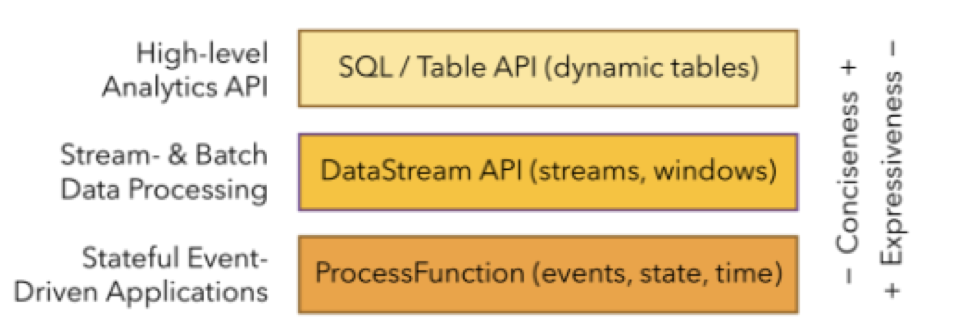
\includegraphics[width=0.9\textwidth]{image11.png}
      \caption{分层API}
    \end{figure}
  
  \end{frame}

  \begin{frame}
    \frametitle{Flink 的其它特点}

    \begin{itemize}
      \item 支持事件时间(event-time)和处理时间(processing-time)语义
      \item 精确一次(exactly-once)的状态一致性保证
      \item 低延迟,每秒处理数百万个事件,毫秒级延迟(实际上就是没有延迟)
      \item 与众多常用存储系统的连接(ES,HBase,MySQL,Redis…)
      \item 高可用(zookeeper),动态扩展,实现7*24小时全天候运行
    \end{itemize}
  
  \end{frame}

  \begin{frame}
    \frametitle{Flink vs Spark Streaming}
  
    \begin{itemize}
      \item 流(stream)和微批
    \end{itemize}
  
  \end{frame}

  \begin{frame}
    \frametitle{Flink vs Spark Streaming}
  
    \begin{itemize}
      \item 数据模型
        \begin{itemize}
          \item Spark采用RDD模型,Spark Streaming的DStream实际上也就是一组组小批数据RDD的集合
          \item Flink基本数据模型是数据流,以及事件(Event)序列(Integer、String、Long、POJO Class)
        \end{itemize}
      \item 运行时架构
        \begin{itemize}
          \item Spark是批计算,将DAG划分为不同的Stage,一个Stage完成后才可以计算下一个Stage
          \item Flink是标准的流执行模式,一个事件在一个节点处理完后可以直接发往下一个节点进行处理
        \end{itemize}
    \end{itemize}
  
  \end{frame}

  \begin{frame}[fragile]
    \frametitle{单词计数程序}
  
    \begin{minted}[linenos,breaklines,fontsize=\footnotesize]{java}
    public static void main(String[] args) throws Exception {
        final StreamExecutionEnvironment env = StreamExecutionEnvironment.getExecutionEnvironment();
        env.setParallelism(1);

        DataStream<String> stream = env.fromElements("Hello World", "Hello World");

        stream
                .flatMap(new Tokenizer())
                .keyBy(r -> r.f0)
                .sum(1)
                .print();

        env.execute("单词计数");
    }
    \end{minted}
  
  \end{frame}

  \begin{frame}[fragile]
    \frametitle{单词计数程序}
  
    \begin{minted}[linenos,breaklines,fontsize=\footnotesize]{java}
    public static class Tokenizer implements FlatMapFunction<String, Tuple2<String, Integer>> {
        @Override
        public void flatMap(String value, Collector<Tuple2<String, Integer>> out) throws Exception {
            String[] stringList = value.split("\\s");
            for (String s : stringList) {
                out.collect(Tuple2.of(s, 1));
            }
        }
    }
    \end{minted}
  
  \end{frame}

  \begin{frame}[plain,c]
    %\frametitle{A first slide}
    
    \begin{center}
    \Huge Q \& A
    \end{center}
    
  \end{frame}

\end{document}
